\subsection{Software Components}

In this section we describe the principal software components and organization of the AZ-SMART system.  AZ-SMART will include three modules (Project Manager, Data Manager, and Tool Manager) based on the AZ-SMART RFQ Appendix G. Each module's organization and implementation are described in turn in the following subsections.

%Projects are defined as the database and model configuration used to support running a variety of scenarios that would share data and model specifications and parameters.  Scenarios are defined as a set of input data, assumptions, and run configuration parameters used for a specific run of the model system.


\subsubsection{Data Manager}

The Data Manager will focus on the management and visualization of data within AZ-SMART.  The Data Manager be implemented within the ArcGIS framework as a dockable window, coded in VB.NET and ArcObjects, that organizes the necessary data management tools in a 'tree-view' framework.  The Data Manager dockable window would be accessible within both ArcMap and ArcCatalog to provide flexibility in use, although in regular production operation it would probably make the most sense to utilize the Data Manager primarily within ArcCatalog.  See figures XXX and XXX for example screen captures of this type of dockable window implementation in both ArcCatalog and ArcMap. 

%\emph{Paul said:...change the reference in the preceding sentence to the Latex reference... Jesse says: I am having trouble getting the figure code in the .tex doc to build properly, so I just inserted the figure as you see here and commented out the figure specific code}

\begin{figure}[h]
\begin{center}
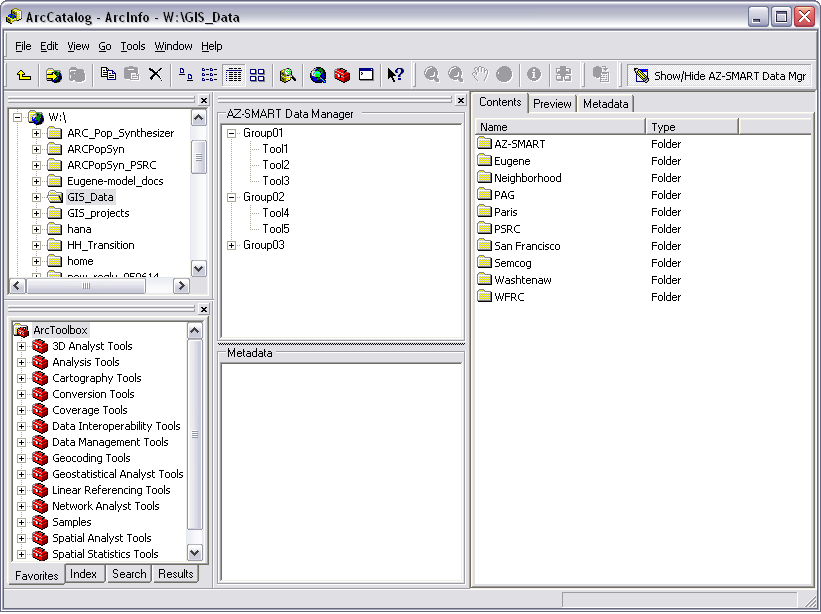
\includegraphics[scale=0.4]{figures/AZ-SMART_DataManager_in_ArcCatalog.png}
\caption{AZ-SMART Data Manager dockable window in ArcCatalog}
\label{figCatalog}
\end{center}
\end{figure}

\begin{figure}[h]
\begin{center}
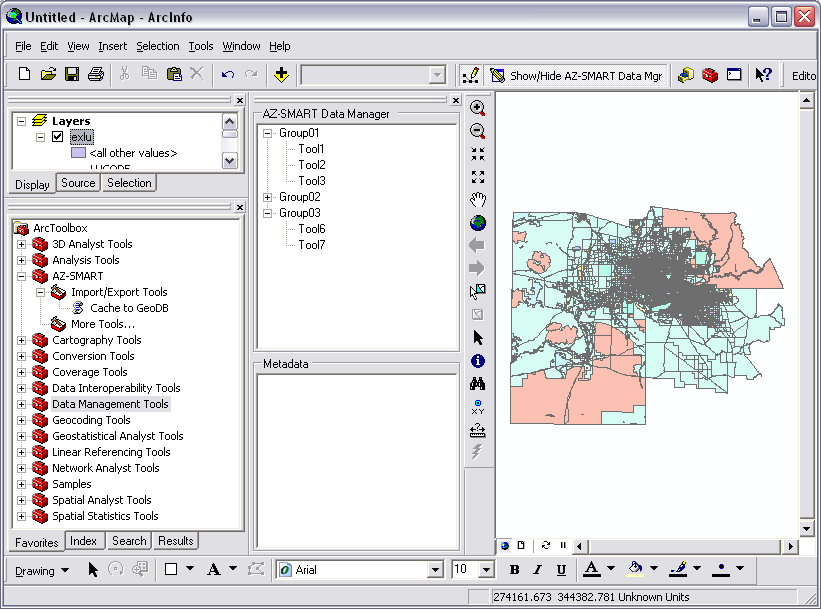
\includegraphics[scale=0.4]{figures/AZ-SMART_DataManager_in_ArcMap.png}
\caption{AZ-SMART Data Manager dockable window in ArcMap}
\label{figMap}
\end{center}
\end{figure}

The Data Manager will focus on metadata maintenance and management, management of security levels and users, data archiving, and the movement of data between the OPUS cache and the geodatabase.  To the greatest extent possible, existing ArcCatalog functionality will be utilized to manage the geodatabase, including managing and maintaining geographic datasets and creating and tracking relationships.

\emph{There is a need to define requirements for metadata, and data archiving in the AZ-SMART system.  Once these requirements are identified we can proceed with devising suitable designs to address these requirements.}

\subsubsection{Tool Manager}

The Tool Manager will focus on the management and execution of the wide variety of tools to be developed for AZ-SMART.  The ArcToolbox/ModelBuilder framework will be used for the organization, management, indexing, and execution of tools.  Specifically, a new AZ-SMART toolbox will be populated with the required tools, which will then be organized into toolsets based on common functionality.  To the greatest extent possible new functionality for AZ-SMART will be developed as Python geoprocessing tools within these toolsets, while minimizing custom GUI development within the ArcMap and ArcCatalog applications.  If the required functionality cannot be implemented in Python through the existing ESRI geoprocessing object and/or other add-on Python libraries, CUSPA will develop custom geoprocessing tools using VB.NET and ArcObjects.

\emph{Jesse: insert appropriate screenshot and reference here.  Can you flesh out an initial list of the tools you think will be needed in this in order to accomplish what we need?  I believe we need more detail here and you should be able to do this from the information you have on SAM and your understanding of how functionality could be accessed via ArcTools.}

\bigskip

List of tools:

\bigskip

\textbf{Data Import/Export Tools:}

\bigskip

Description: OPUS Cache to Geodatabase

Purpose: Convert a single attribue, table, or entire cache to a Geodatabase

Implementation: Traits/UI dialog box run from AZ-SMART Toolbox or OPUS GUI

\bigskip

Description: Geodatabase to OPUS Cache

Purpose: Convert all or part of an attribute table from a Geodatabase to the OPUS Cache

Implementation: Traits/UI dialog box run from AZ-SMART Toolbox or OPUS GUI

\bigskip

Description: OPUS Cache to ASCII table

Purpose: Convert OPUS Cache to ASCII table on disk (e.g. .csv, .tab, etc.)

Implementation: Traits/UI dialog box run from AZ-SMART Toolbox or OPUS GUI

\bigskip

Description: Geodatabase to ASCII table

Purpose: Convert ll or part of an attribute table from a Geodatabase to an ASCII table

Implementation: Traits/UI dialog box run from AZ-SMART Toolbox or OPUS GUI

\bigskip

Description: OPUS Cache to DBASE table

Purpose: Convert OPUS Cache table to DBASE table

Implementation: Traits/UI dialog box run from AZ-SMART Toolbox or OPUS GUI

\bigskip

Description: Geodatabase to DBASE table

Purpose: Convert Geodatabase table to DBASE table

Implementation: Traits/UI dialog box run from AZ-SMART Toolbox or OPUS GUI

\bigskip

Description: OPUS Cache to Excel table

Purpose: Convert OPUS Cache table to Excel table

Implementation: Traits/UI dialog box run from AZ-SMART Toolbox or OPUS GUI

\bigskip

Description: Geodatabae to Excel table

Purpose: Convert Geodatabase table to Excel table

Implementation: Traits/UI dialog box run from AZ-SMART Toolbox or OPUS GUI

\bigskip

Description: Excel table to Geodatabase

Purpose: Convert Excel table to Geodatabase table

Implementation: Traits/UI dialog box run from AZ-SMART Toolbox or OPUS GUI

\bigskip

Description: Excel table to OPUS Cache

Purpose: Convert Excel table to OPUS Cache

Implementation: Traits/UI dialog box run from AZ-SMART Toolbox or OPUS GUI

\bigskip

\textbf{Indicator Tools:}

\bigskip

Description: Generate Spatial Indicator(s)

Purpose: To read the OPUS cache and generate a spatial indicator for viewing in ArcMap

Implementation: Traits/UI dialog box run from AZ-SMART Toolbox or OPUS GUI

\bigskip

Description: Generate Spatial Indicator Map(s)

Purpose: To read the OPUS Cache and generate a complete map based on a map template

Implementation: Traits/UI dialog box run from AZ-SMART Toolbox or OPUS GUI

\bigskip

Description: Generate Indicator Graph/Chart

Purpose: To generate a graph or chart based on an indicator over specified years

Implementation: Traits/UI dialog box run from AZ-SMART Toolbox or OPUS GUI

\bigskip

Description: Generate Report

Purpose: To generate a document that consists of Spatial Indicator Maps and Graphs

Implementation: Traits/UI dialog box run from AZ-SMART Toolbox or OPUS GUI

\bigskip

\textbf{Aggregation/Disaggregation Tools:}

\bigskip

Description: Aggregate to Geography

Purpose: Aggregate a theme to a larger polygon geography

Implementation: Standard ArcToolbox GUI

\bigskip

Description: Disaggregate to Geography

Purpose: Disaggregate a theme to a smaller polygon geography (based on percent area)

Implementation: Standard ArcToolbox GUI

\bigskip

\textbf{Model Estimation Tools}

Description: Estimate Regression Model

Purpose: Tool to estimate a standard regression model

Implementation: Traits/UI dialog box run from AZ-SMART Toolbox or OPUS GUI

\bigskip

Description: Estimate Logit Model

Purpose: Tool to estimate a logit model

Implementation: Traits/UI dialog box run from AZ-SMART Toolbox or OPUS GUI

\bigskip

\textbf{Run Configuration Tools}

\bigskip

\textbf{Data Diagnostic Tools}

\bigskip

Description: Descriptive Statistics

Purpose: Reports descriptive statistics for attributes in a data table(s) (OPUS cache or geodatabase)

Implementation: Traits/UI dialog box run from AZ-SMART Toolbox or OPUS GUI

\bigskip

Description: Variable Distribution

Purpose: Produces graphics of the distribution of variables (OPUS cache or geodatabase)

Implementation: Traits/UI dialog box run from AZ-SMART Toolbox or OPUS GUI

\bigskip

Description: Data Diagnostic Report

Purpose: Produces a document that consists of multiple Descriptive Statistics and Variable Distributions

Implementation: Traits/UI dialog box run from AZ-SMART Toolbox or OPUS GUI

\bigskip

\textbf{Data Imputation Tools}

\bigskip

Description: Impute average/most-frequent value

Purpose: Fills in missing values with the average (for continuous variable) or most frequent (for discrete)

Implementation: Traits/UI dialog box run from AZ-SMART Toolbox or OPUS GUI

\bigskip

Description: Impute random value

Purpose: Fills in missing values with a random value (within a specified or computed range)

Implememtation: Traits/UI dialog box run from AZ-SMART Toolbox or OPUS GUI

\bigskip

Description: Impute via model

Purpose: Fills in missing values based on a specified model

Implementation: Traits/UI dialog box run from AZ-SMART Toolbox or OPUS GUI

\bigskip

\subsubsection{Land Use Editor}
When SAM-IM was develped in the ArcView environment, there was considerable functionality not present in the underlying GIS platform that needed to be developed in SAM-IM, such as editing of polygons.  In the development of AZ-SMART on the ArcGIS 9.x platform, there is no need to develop such functionality, since editing tools for spatial data are built-in.  The initial plan for AZ-SMART is to maximize the use of built-in functionality and minimize the amount of custom-code development which will need to be maintained and synchronized with evolving ArcGIS functionality and interfaces.  If it becomes clear that there is some need for customization of the built-in functionality for editing after the AZ-SMART system is put into testing and use, specifications for this could be developed and the task prioritized along with other tasks in the project.

%\emph{Note from Jesse:  we may need other customizations within ArcGIS to accomplish what they want in App G.  For instance, they desribe a land use editor that may require some custom GUI development.  Should we attempt to describe those here? }

\subsubsection{Project Manager}

The Project Manager will focus on managing the model components of the system. The Project Manager will leverage and manage modeling infrastructure embeded in the OPUS system, and will take advantage of the run management capabilities of OPUS such as model specification, estimation, execution, and generation of indicators.  The Project Manager user interface would be accessible from within ArcGIS, and will open a windowed application which we refer to as the OPUS GUI.  The OPUS GUI, developed in Python and using the Envisage tools from Enthought, could also be used outside of ArcGIS, providing flexibility for a range of use cases.  The Project Manager will be the central application where simulation runs are configured, managed, started and stopped, and will interoperate seamlessly with the Data Manager and Tol Manager components of AZ-SMART.

Several of the items listed in the Project Manager requirements in AZ-SMART RFQ Appendix G are very focused on control of model operations: controlling model execution, accessing the status of a model while executing, and accessing execution logs and error logs associated with a model run.  Compared to an approach of using only native ArcGIS GUI tools to code the Project Manager, the approach of coding a native OPUS GUI will make it more feasible to implement these requirements.  It would need to be implemented in a way that could inter-operate transparently with other tools in the Tool Manager and Data Manager components, as noted in the first requirement below. Some initial tests of this approach should be developed early in the project to flesh out this aspect of the user interface.

